\documentclass{article}
\usepackage{color}
\usepackage{placeins}
\usepackage{listings}
\usepackage{graphicx}
\usepackage{xcolor}
\usepackage{amsmath}
\usepackage{subcaption}
\usepackage{cleveref}
\usepackage{array}
\usepackage{geometry}[margins=1in]
\setlength{\parskip}{4pt plus 2pt}
\setlength{\parindent}{0pt}
%\pagecolor[rgb]{0,0,0} %black
%\color[rgb]{1,1,1} %grey
\lstset{language=C++,
keywordstyle=\color{blue},
stringstyle=\color{red},
commentstyle=\color{green},
morecomment=[l][\color{magenta}]{\#},
breaklines=true,
breakatwhitespace=true,
numbers=left
}
\title{Assignment \#5}
\author{Asbjørn Bonefeld Preuss,\\ Daniel Lomholt Christensen,\\ Elie Cueto}
\date{March 2024}

\renewcommand{\thesection}{Task \#\arabic{section}}
\renewcommand{\thesubsection}{\arabic{section}.\arabic{subsection}}
\begin{document}
\maketitle
\section{OpenACC parallelise the program}
The initial bottlenecks of the program without OpenACC was analysed using gprof. The result can be seen in figure \ref{fig:profiling:seq}. The profiling showed that efforts at parallelising the program should be focused around the integration function.
\begin{figure}
    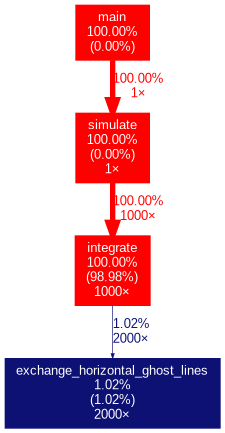
\includegraphics[width=0.3\textwidth]{./figures/sequential_profile.png}
    \centering
    \caption{Profiling of the sequential code, run with gprof and generated with gprof2dot.}
    \label{fig:profiling:seq}
\end{figure}
We initially had some loops running in parallel on the gpu. 
We did this by initialising a GPU accelerated region around the for loop of the simulation (line 155-164).
We here define which data is copied in, and must be copied out as well. In this function, the calculated version of water\_world.e is pushed to the cpu's version of water\_history.

On line 158 the integration function is called. In the integration function, the exchange horizontal and vertical ghost lines functions were quickly paralellised with acc parallel loop gang directives.

Next up, the integration function has two nested for loops, that are parallelized with parallel loop collapse.

With this setup we profiled the GPU accelerated code, and this result can be seen in table \ref{tab:nvsys_profiling}. This initial attempt highlights that most of the time for the cpu is spent polling and waiting for the GPU to return with an answer, i.e the GPU is definitely doing the heavy lifting.

In the next attempt at optimization, we merged the two horizontal ghost line functions, as well as the two vertical ghost line functions, such that they calculate both w.e and w.u at the same time.

The initialisation of the accelerated region was also changed, such that it only copies in, not out. Finally, the integration loops gained an extra level of parallelisation by becoming parallel loop gang vectors instead of just parallel loops. This allows these used to be executed by gangs in vectors.

The profiling results from this implementation can also be seen in table \ref{tab:nvsys_profiling}. The difference between the last attempt and this one, seems to be that more time is spent waiting for the gpu to finish, but this may just be within the statistical uncertainties, as seen by the standard deviation of the time spent waiting compared to the average time.

\begin{table}
    \centering
    \begin{tabular}{|m{0.2\textwidth}|m{0.2\textwidth}|m{0.2\textwidth}|m{0.2\textwidth}|m{0.15\textwidth}|}
    \hline
       Version of the code  & Functions that use the most time & The time they use \% & avg time spent in the function[ms] & stddev of time spent in function[ms]\\
       \hline
       1  & sem\_wait & 41.7\% & 274.4 & 361.1\\
         & poll & 32.7\% & 26.9& 34.3\\
         & ioctl & 12.3\% & 0.3& 1.63\\
         \hline
        2  & sem\_wait & 46.4\% & 292.1& 393.7\\
         & poll & 34.1\% & 26.9& 36.1\\
         & ioctl & 15.1\% & 0.3& 1.7\\
         \hline
        3  & sem\_wait & 48.4\% & 5330.7& 7505.6\\
         & poll & 47.9\% & 90.1& 27.37\\
         & writev & 2.3\% & 501.5& 0\\
         \hline
         
    \end{tabular}
    \caption{nvsys profiling outputs from the different versions of the code. sem\_wait is the cpu waiting for }
    \label{tab:nvsys_profiling}
\end{table}

The third attempt focused on directing the compiler as to what data is already present on the GPU. This was done by the use of the present(variables) clause, which was put into the ghost functions, as well as the integration function.

Furthermore, the division of dt/dx and dt/dy in the integration function, was calculated a priori, such that we save those flops.

A profiling of this third attempt can also be seen in table \ref{tab:nvsys_profiling}. This final attempt seems to have had its profiling somewhat muddled by a specific sem\_wait call, as the avg time spent in sem\_wait is 70\% of the standard deviation of time spent in sem\_wait calls...

The final attempt at optimising the code laid in only sending water\_history forth and back once between CPU and GPU, as well as parallelising a larger region at once, resulting in us optimising the synchronisation effort between individual GPU loops and the CPU, out of the program. This however did not work, and has thus not been included in this report.

\section{Strong and weak scaling using SLURM}
Here we first test the strong scaling of the code. We do this by running each of the three versions of our code described above with $NX=NY=4096$. We vary the number of gangs between $1$ and $141$ in steps of $5$, and run the codes six times for each number of gangs to get better statistics on the runtimes. We keep the vector length constant at $128$ throughout. The results of this is shown in figure \ref{fig:strong}, along with fits to Amdahls law. All three versions of the code run very similarly well, and have very similar serial fractions of $\sim0.02$. Additionally, all three versions of the code perform significantly worse and significantly less consistently when the number of gangs is raised above $125$. At this point it seems that the cost of having many gangs scheduled at once comes to exceed the improvement in latency from not having to wait for new instructions. Below this point, however the codes scale very similarly to what would be expected from Amdahl's law.

Next up, we test the weak scaling capabilities of the code. Here we vary the grid length in steps of $512$ between $1024$ and $7680$. As the size of the system (and the number of computations) scales quadratically with the grid length, we also increase the number of gangs quadratically from $2$ at $NX=1024$ to $112$ at $NX=7680$. We still keep the vector length constantat $128$. We test the scaling in the same way described above and the speed-up is shown in figure \ref{fig:weak}. This is not quite as pretty as the strong scaling, but we do see significant speed-up when scaling up the size of the problem. The best speed-up seems to be achieved at around $70-80$ gangs, with $NX=6144-6656$. We do, however, have a significant variation in runtime even when testing each version $8$ times, so it is not entirely clear where the best speed-up is obtained. That said the weak scaling does show that performance drops off at the largest scales we tested.
\begin{figure}
    \centering
    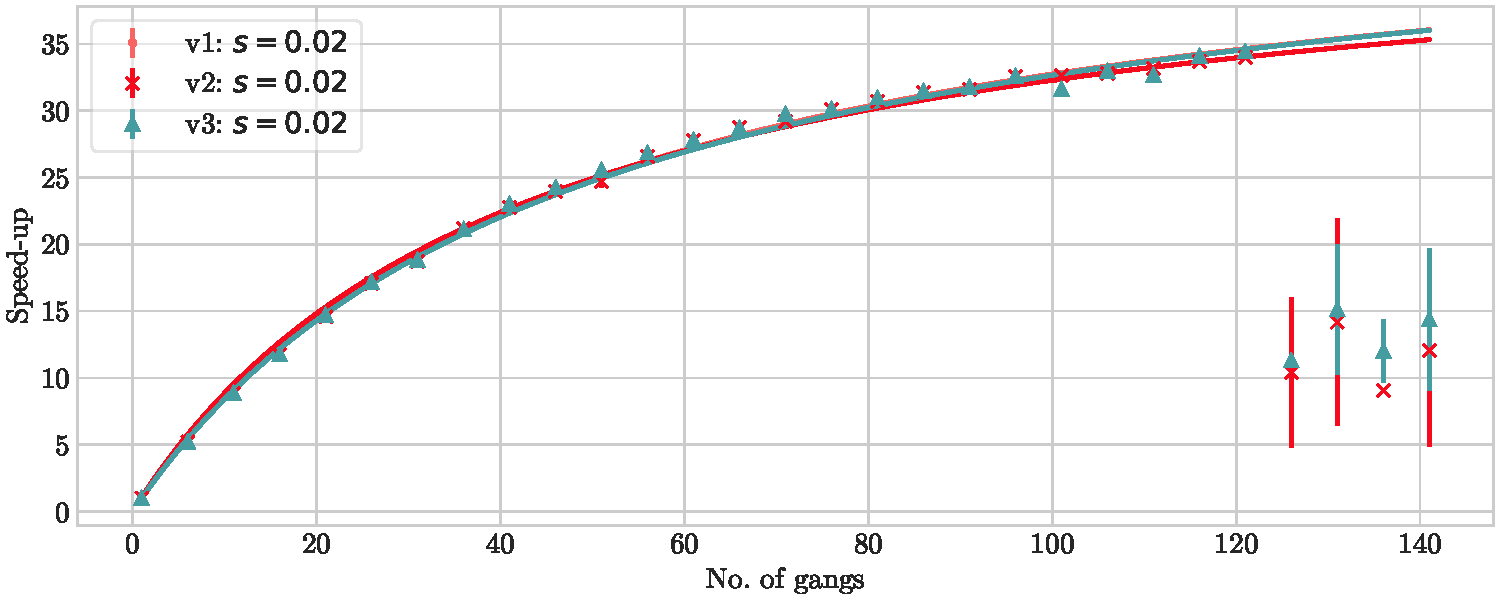
\includegraphics[width=\textwidth]{Assignment_5_shallow_water/Report/figures/amdahl.pdf}
    \caption{Strong scaling for the three different versions of the code and fits to Amdahls law to determine Serial fraction of the code. For each version the serial fraction is about $0.02$}
    \label{fig:strong}
\end{figure}
\begin{figure}
    \centering
    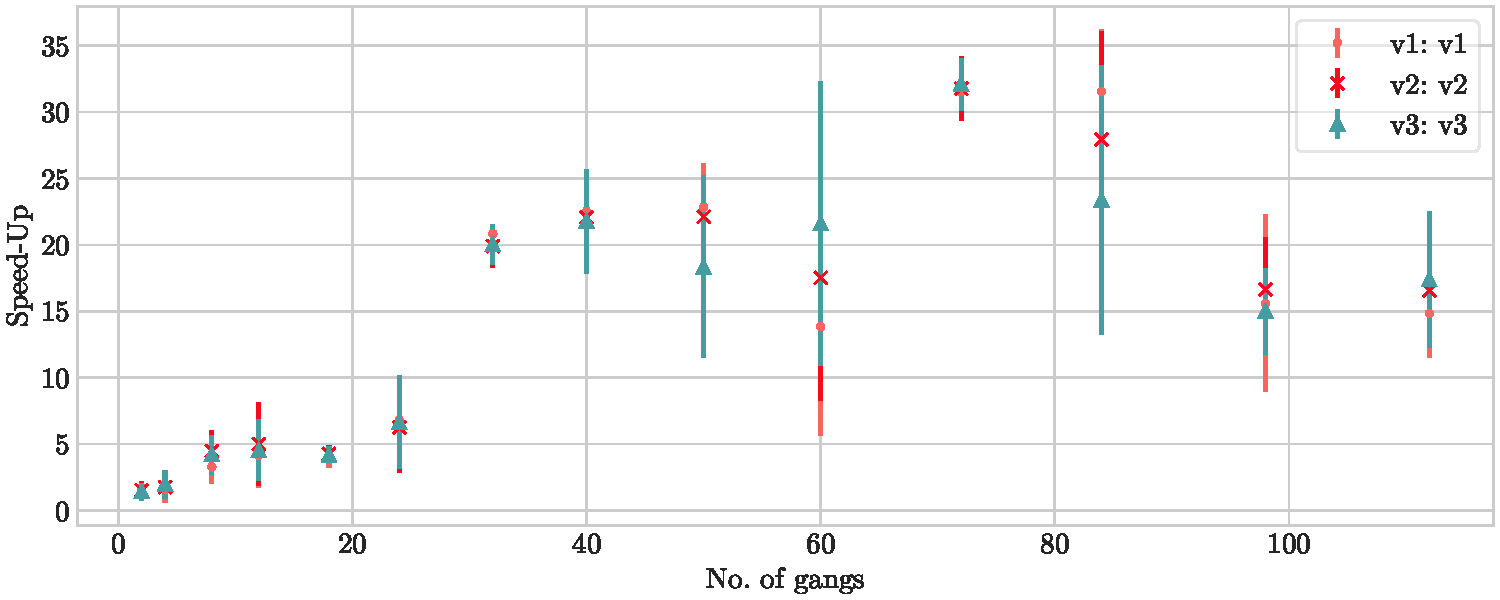
\includegraphics[width=\textwidth]{Assignment_5_shallow_water/Report/figures/weak_scaling_corrected.pdf}
    \caption{Weak scaling for the three different versions of the code}
    \label{fig:weak}
\end{figure}


\FloatBarrier
\section{Source Code}
\label{sec:source}
\lstinputlisting[language=c++]{../Code/sw_parallel.cpp}

\end{document}
